\documentclass{article}
\usepackage{amssymb,amsmath}
\usepackage{ifxetex,ifluatex}
\ifxetex
  \usepackage{fontspec,xltxtra,xunicode}
  \defaultfontfeatures{Mapping=tex-text,Scale=MatchLowercase}
\else
  \ifluatex
    \usepackage{fontspec}
    \defaultfontfeatures{Mapping=tex-text,Scale=MatchLowercase}
  \else
    \usepackage[utf8]{inputenc}
  \fi
\fi
\usepackage{graphicx}
% We will generate all images so they have a width \maxwidth. This means
% that they will get their normal width if they fit onto the page, but
% are scaled down if they would overflow the margins.
\makeatletter
\def\maxwidth{\ifdim\Gin@nat@width>\linewidth\linewidth
\else\Gin@nat@width\fi}
\makeatother
\let\Oldincludegraphics\includegraphics
\renewcommand{\includegraphics}[1]{\Oldincludegraphics[width=\maxwidth]{#1}}
\ifxetex
  \usepackage[setpagesize=false, % page size defined by xetex
              unicode=false, % unicode breaks when used with xetex
              xetex]{hyperref}
\else
  \usepackage[unicode=true]{hyperref}
\fi
\hypersetup{breaklinks=true, pdfborder={0 0 0}}
\setlength{\parindent}{0pt}
\setlength{\parskip}{6pt plus 2pt minus 1pt}
\setlength{\emergencystretch}{3em}  % prevent overfull lines
\setcounter{secnumdepth}{0}

\title{Correlations}
\author{(Username not set) (E-mail address not set)}
\date{2011--04--26 20:25 CET}

\begin{document}
\maketitle

\subsection{Description}

This template will return the correlation matrix of supplied numerical
variables.

\subsubsection{Variable description}

3 variables provided.

The highest correlation coefficient (0.2364) is between ``it.edu'' and
``age'' and the lowest (--0.049) is between ``it.leisure'' and ``age''.
It seems that the strongest association (r=0.2364) is between ``it.edu''
and ``age''.

Higly correlated (r \textless{} 0.7 or r \textgreater{} 0.7) variables:
-

Uncorrelated (--0.2 \textless{} r \textless{} 0.2) variables: * ``age''
- ``it.leisure'' * ``it.edu'' - ``it.leisure''

\paragraph{Correlation matrix}

\begin{figure}[htbp]
\centering
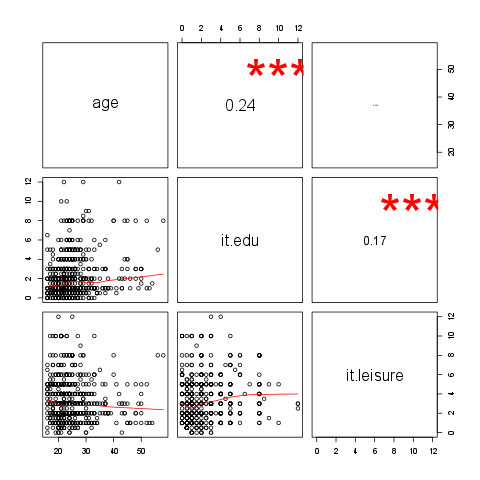
\includegraphics{7abdf648965ac14c778c4d61dddc7023.png}
\caption{}
\end{figure}

\end{document}
